\documentclass[tikz,border=2pt,11pt]{standalone}
\usetikzlibrary{arrows.meta}
\usetikzlibrary{calc}
\usetikzlibrary{positioning}
\usepackage{amsmath}
\usepackage{amssymb}
\usepackage{mathrsfs}
\usepackage{xcolor}
\usepackage{tikz}
\newcommand{\C}{\mathbb C}
\newcommand{\R}{\mathbb R}
\newcommand{\Z}{\mathbb Z}
\newcommand{\N}{\mathbb N}
\newcommand{\E}{\mathbb E}
\newcommand{\Prob}{\mathbb P}
\DeclareMathOperator{\diam}{diam}
\DeclareMathOperator{\tr}{tr}
\DeclareMathOperator{\supp}{supp}
\DeclareMathOperator{\dist}{dist}
\DeclareMathOperator{\Var}{Var}
\newcommand{\MathActualText}[2]{
  \BeginAccSupp{method=hex,unicode,ActualText=#1}
  #2
  \EndAccSupp{}
}
\renewcommand{\mapsto}{\mathrel{\MathActualText{21A6}{\OriginalMapsto}}}
\renewcommand{\hookrightarrow}{\mathrel{\MathActualText{21AA}{\OriginalHookrightarrow}}}
\renewcommand{\longrightarrow}{\mathrel{\MathActualText{27F6}{\OriginalLongrightarrow}}}
\begin{document}
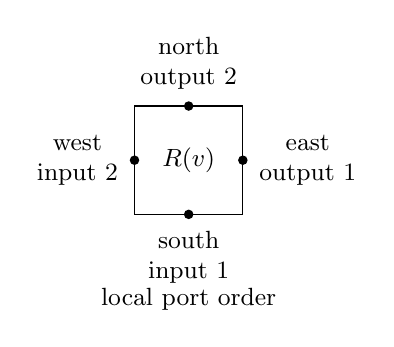
\begin{tikzpicture}[scale=.86,every node/.style={font=\small}]
 \draw (-.8,-.8) rectangle (.8,.8);
 \node at (0,0) {$R(v)$};
 \foreach \x/\y in {0/-.8,-.8/0,.8/0,0/.8}
    \fill (\x,\y) circle (2pt);
 \node[below,align=center] at (0,-.9) {south\\input 1};
 \node[left,align=center] at (-.9,0) {west\\input 2};
 \node[right,align=center] at (.9,0) {east\\output 1};
 \node[above,align=center] at (0,.9) {north\\output 2};
 \node at (0,-2.05) {local port order};
\end{tikzpicture}
\end{document}
